\documentclass[12pt,a4paper]{report}
\usepackage[T2A]{fontenc}
\usepackage[utf8]{inputenc}
\usepackage[russian]{babel}
\usepackage{graphicx, setspace, amsmath}


\usepackage[
top = 1.25cm,
bottom = 2.0cm]{geometry}

\begin{document}
\begin{titlepage}
	\centering
    % HEADER
	{
        \scshape
        Федеральное государственное автономное образовательное учреждение высшего образования
        \par
        \textbf{«Научно-образовательная корпорация ИТМО»}
        \par
        \vspace*{1cm}
        Факультет Программной Инженерии и Компьютерной Техники
        \par
    }
    % LOGO
    \vspace*{0.6cm}
    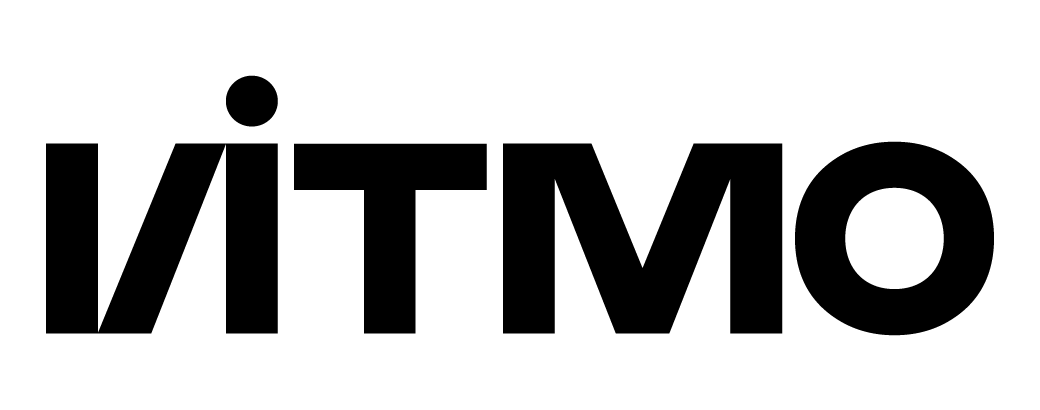
\includegraphics[width=\textwidth]{logo.png}
    % LAB INFO
    {
        \Large
        \textbf{Домашняя работа по представлению чисел в ЭВМ №2}
        \par
        \normalsize
        \vspace*{0.75cm}
        \textbf{Вариант 43}
        \par
    }
    \vfill
    % СREDITS
    \hfill\begin{minipage}{\dimexpr\textwidth-7.8cm}
        \textbf{Выполнил:}\par
        Степанов Арсений Алексеевич\par
        \vspace*{0.15cm}
        \textbf{Группа:}\par
        P3109\par
        \vspace*{0.15cm}
        \textbf{Преподаватель:}\par
        Поляков Владимир Иванович\par
    \end{minipage}
    \vfill
    Санкт-Петербург, \the\year{}г.
\end{titlepage}
\section*{Значения чисел для данного варианта}
\onehalfspacing
$A=81_{10}=01010001_2$\\
$-A=10101111_2$\\
$B=36_{10}=00100100_2$\\
$-B=11011100_2$
\section*{Задание №1}
\begin{tabular}{cccc} % Part 1
    \begin{tabular}{c}
        A > 0, B > 0\\
        $
        \large
        \begin{array}{r}
        +
        \begin{array}{r}
        01010001\\
        00100100\\
        \end{array} \\
        \hline
        \begin{array}{r}
        01110101
        \end{array}
        \end{array}
        $
    \end{tabular} &
    \begin{tabular}{c}
        З.И.\\
        $
        \large
        \begin{array}{r}
        +
        \begin{array}{r}
        81\\
        36\\
        \end{array} \\
        \hline
        \begin{array}{r}
        117
        \end{array}
        \end{array}
        $
    \end{tabular} &
    \begin{tabular}{c}
        Б.З.И.\\
        $
        \large
        \begin{array}{r}
        +
        \begin{array}{r}
        81\\
        36\\
        \end{array} \\
        \hline
        \begin{array}{r}
        117
        \end{array}
        \end{array}
        $
    \end{tabular} &
    \begin{tabular}{ccc}
    CF$=0$ & PF$=0$ & AF$=0$\\
    ZF$=0$ & SF$=0$ & OF$=0$
    \end{tabular}
\end{tabular}
\hfill\break
\vspace*{1cm}
\hfill\break
\begin{tabular}{cccc} % Part 2
    \begin{tabular}{c}
        A < 0, B > 0\\
        $
        \large
        \begin{array}{r}
        +
        \begin{array}{r}
        1\overset{\normalsize{1}}{0}1\overset{\normalsize{1}}{0}\overset{\normalsize{1}}{1}111\\
        00100100\\
        \end{array} \\
        \hline
        \begin{array}{r}
        C_{com}\;\;11010011
        \end{array}\\
        \hline
        \begin{array}{r}
        C_{dir}\;\;00101101
        \end{array}\\
        \end{array}
        $
    \end{tabular} &
    \begin{tabular}{c}
        З.И.\\
        $
        \large
        \begin{array}{r}
        +
        \begin{array}{r}
        -81\\
        36\\
        \end{array} \\
        \hline
        \begin{array}{r}
        -45
        \end{array}\\
        \hline
        \begin{array}{r}
        *
        \end{array}\\
        \end{array}
        $
    \end{tabular} &
    \begin{tabular}{c}
        Б.З.И.\\
        $
        \large
        \begin{array}{r}
        +
        \begin{array}{r}
        175\\
        36\\
        \end{array} \\
        \hline
        \begin{array}{r}
        *
        \end{array}\\
        \hline
        \begin{array}{r}
        211
        \end{array}\\
        \end{array}
        $
    \end{tabular} &
    \begin{tabular}{ccc}
    CF$=0$ & PF$=0$ & AF$=1$\\
    ZF$=0$ & SF$=1$ & OF$=0$
    \end{tabular}
\end{tabular}
\hfill\break
\vspace*{1cm}
\hfill\break
\begin{tabular}{cccc} % Part 3
    \begin{tabular}{c}
        A > 0, B < 0\\
        $
        \large
        \begin{array}{r}
        +
        \begin{array}{r}
        \overset{\normalsize{1}}{\phantom{0}}\overset{\normalsize{1}}{0}1\overset{\normalsize{1}}{0}10001\\
        11011100\\
        \end{array} \\
        \hline
        \begin{array}{r}
        00101101
        \end{array}
        \end{array}
        $
    \end{tabular} &
    \begin{tabular}{c}
        З.И.\\
        $
        \large
        \begin{array}{r}
        +
        \begin{array}{r}
        81\\
        -36\\
        \end{array}\\
        \hline
        \begin{array}{r}
        45
        \end{array}
        \end{array}
        $
    \end{tabular} &
    \begin{tabular}{c}
        Б.З.И.\\
        $
        \large
        \begin{array}{r}
        +
        \begin{array}{r}
        81\\
        230\\
        \end{array}\\
        \hline
        \begin{array}{r}
        45?
        \end{array}\\
        \end{array}
        $
    \end{tabular} &
    \begin{tabular}{ccc}
    CF$=1$ & PF$=0$ & AF$=0$\\
    ZF$=0$ & SF$=0$ & OF$=0$
    \end{tabular}
\end{tabular}
\hfill\break
Результат неверен для беззнаковой интерпретации, так как полученное число не умещается в формат\\
\hfill\break
\begin{tabular}{cccc} % Part 4
    \begin{tabular}{c}
        A < 0, B < 0\\
        $
        \large
        \begin{array}{r}
        +
        \begin{array}{r}
        \overset{\normalsize{1}}{\phantom{0}}\overset{\normalsize{1}}{1}\overset{\normalsize{1}}{0}\overset{\normalsize{1}}{1}\overset{\normalsize{1}}{0}\overset{\normalsize{1}}{1}111\\
        11011100\\
        \end{array} \\
        \hline
        \begin{array}{r}
        C_{com}\;\;10001011
        \end{array}\\
        \hline
        \begin{array}{r}
        C_{dir}\;\;01110101
        \end{array}\\
        \end{array}
        $
    \end{tabular} &
    \begin{tabular}{c}
        З.И.\\
        $
        \large
        \begin{array}{r}
        +
        \begin{array}{r}
        -81\\
        -36\\
        \end{array} \\
        \hline
        \begin{array}{r}
        -117
        \end{array}\\
        \hline
        \begin{array}{r}
        *
        \end{array}\\
        \end{array}
        $
    \end{tabular} &
    \begin{tabular}{c}
        Б.З.И.\\
        $
        \large
        \begin{array}{r}
        +
        \begin{array}{r}
        175\\
        230\\
        \end{array} \\
        \hline
        \begin{array}{r}
        *
        \end{array}\\
        \hline
        \begin{array}{r}
        117?
        \end{array}\\
        \end{array}
        $
    \end{tabular} &
    \begin{tabular}{ccc}
    CF$=1$ & PF$=1$ & AF$=1$\\
    ZF$=0$ & SF$=1$ & OF$=0$
    \end{tabular}
\end{tabular}
\hfill\break
Результат неверен для беззнаковой интерпретации, так как полученное число не умещается в формат\\
\hfill\break
\section*{Задание №2}
$B'=66_{10}=01000010_2$\\
$-B'=-66_{10}=10111110_2$\\
\hfill\break
\begin{tabular}{cccc} % Part 5
    \begin{tabular}{c}
        A > 0, B > 0\\
        $
        \large
        \begin{array}{r}
        +
        \begin{array}{r}
        \overset{\normalsize{1}}{0}1010001\\
        01000010\\
        \end{array} \\
        \hline
        \begin{array}{r}
        C_{com}\;\;10010011
        \end{array}\\
        \hline
        \begin{array}{r}
        C_{dir}\;\;01101101
        \end{array}\\
        \end{array}
        $
    \end{tabular} &
    \begin{tabular}{c}
        З.И.\\
        $
        \large
        \begin{array}{r}
        +
        \begin{array}{r}
        81\\
        66\\
        \end{array} \\
        \hline
        \begin{array}{r}
        -109?
        \end{array}\\
        \hline
        \begin{array}{r}
        *
        \end{array}\\
        \end{array}
        $
    \end{tabular} &
    \begin{tabular}{c}
        Б.З.И.\\
        $
        \large
        \begin{array}{r}
        +
        \begin{array}{r}
        81\\
        66\\
        \end{array} \\
        \hline
        \begin{array}{r}
        *
        \end{array}\\
        \hline
        \begin{array}{r}
        147
        \end{array}\\
        \end{array}
        $
    \end{tabular} &
    \begin{tabular}{ccc}
    CF$=0$ & PF$=1$ & AF$=0$\\
    ZF$=0$ & SF$=1$ & OF$=1$
    \end{tabular}
\end{tabular}
\hfill\break
Результат неверен для знаковой интерпретации, так как при получении числа произошло переполнение формата\\
\hfill\break
\begin{tabular}{cccc} % Part 6
    \begin{tabular}{c}
        A > 0, B < 0\\
        $
        \large
        \begin{array}{r}
        +
        \begin{array}{r}
        \overset{\normalsize{1}}{\phantom{0}}\overset{\normalsize{1}}{0}\overset{\normalsize{1}}{1}\overset{\normalsize{1}}{0}10001\\
        10111110\\
        \end{array} \\
        \hline
        \begin{array}{r}
        00001111
        \end{array}
        \end{array}
        $
    \end{tabular} &
    \begin{tabular}{c}
        З.И.\\
        $
        \large
        \begin{array}{r}
        +
        \begin{array}{r}
        81\\
        -66\\
        \end{array} \\
        \hline
        \begin{array}{r}
        15
        \end{array}
        \end{array}
        $
    \end{tabular} &
    \begin{tabular}{c}
        Б.З.И.\\
        $
        \large
        \begin{array}{r}
        +
        \begin{array}{r}
        81\\
        190\\
        \end{array} \\
        \hline
        \begin{array}{r}
        15?
        \end{array}
        \end{array}
        $
    \end{tabular} &
    \begin{tabular}{ccc}
    CF$=1$ & PF$=1$ & AF$=0$\\
    ZF$=0$ & SF$=0$ & OF$=0$
    \end{tabular}
\end{tabular}
\hfill\break
Результат неверен для беззнаковой интерпретации, так как полученное число не умещается в формат\\
\section*{Задание №3}
$A'=92_{10}=01011100_2$\\
$A'=-92_{10}=10100100_2$\\
\hfill\break
\begin{tabular}{cccc} % Part 7
    \begin{tabular}{c}
        A > 0, B > 0\\
        $
        \large
        \begin{array}{r}
        +
        \begin{array}{r}
            \overset{\normalsize{1}}{0}\overset{\normalsize{1}}{1}\overset{\normalsize{1}}{0}\overset{\normalsize{1}}{1}\overset{\normalsize{1}}{1}100\\
        00100100\\
        \end{array} \\
        \hline
        \begin{array}{r}
        C_{com}\;\;10000000
        \end{array}\\
        \hline
        \begin{array}{r}
        C_{dir}\;\;10000000
        \end{array}\\
        \end{array}
        $
    \end{tabular} &
    \begin{tabular}{c}
        З.И.\\
        $
        \large
        \begin{array}{r}
        +
        \begin{array}{r}
        92\\
        36\\
        \end{array} \\
        \hline
        \begin{array}{r}
        -128?
        \end{array}\\
        \hline
        \begin{array}{r}
        *
        \end{array}\\
        \end{array}
        $
    \end{tabular} &
    \begin{tabular}{c}
        Б.З.И.\\
        $
        \large
        \begin{array}{r}
        +
        \begin{array}{r}
        92\\
        36\\
        \end{array} \\
        \hline
        \begin{array}{r}
        *
        \end{array}\\
        \hline
        \begin{array}{r}
        128
        \end{array}\\
        \end{array}
        $
    \end{tabular} &
    \begin{tabular}{ccc}
    CF$=0$ & PF$=0$ & AF$=1$\\
    ZF$=0$ & SF$=1$ & OF$=1$
    \end{tabular}
\end{tabular}
\hfill\break
Результат неверен для знаковой интерпретации, так как при получении числа произошло переполнение формата\\
\hfill\break
\begin{tabular}{cccc} % Part 8
    \begin{tabular}{c}
        A < 0, B < 0\\
        $
        \large
        \begin{array}{r}
        +
        \begin{array}{r}
        \overset{\normalsize{1}}{\phantom{0}}\overset{\normalsize{1}}{1}\overset{\normalsize{1}}{0}\overset{\normalsize{1}}{1}\overset{\normalsize{1}}{0}\overset{\normalsize{1}}{0}100\\
        11011100\\
        \end{array} \\
        \hline
        \begin{array}{r}
        C_{com}\;\;10000000
        \end{array}\\
        \hline
        \begin{array}{r}
        C_{dir}\;\;10000000
        \end{array}\\
        \end{array}
        $
    \end{tabular} &
    \begin{tabular}{c}
        З.И.\\
        $
        \large
        \begin{array}{r}
        +
        \begin{array}{r}
        -92\\
        -36\\
        \end{array} \\
        \hline
        \begin{array}{r}
        -128
        \end{array}\\
        \hline
        \begin{array}{r}
        *
        \end{array}\\
        \end{array}
        $
    \end{tabular} &
    \begin{tabular}{c}
        Б.З.И.\\
        $
        \large
        \begin{array}{r}
        +
        \begin{array}{r}
        164\\
        220\\
        \end{array} \\
        \hline
        \begin{array}{r}
        *
        \end{array}\\
        \hline
        \begin{array}{r}
        128?
        \end{array}\\
        \end{array}
        $
    \end{tabular} &
    \begin{tabular}{ccc}
    CF$=1$ & PF$=0$ & AF$=1$\\
    ZF$=0$ & SF$=1$ & OF$=0$
    \end{tabular}
\end{tabular}
\hfill\break
Результат неверен для беззнаковой интерпретации, так как полученное число не умещается в формат\\
\hfill\break
\end{document}